\actTitle{3.3 - Logarithmic Functions}

\noindent \textbf{Topics:}  exponential functions, compound interest, the number $e$, exponential functions with base $e$, growth and decay\\

\noindent \textbf{Student Learning Outcomes:}
\begin{enumerate}
\item Students will be able to recognize a logarithic function graphically and algebraically.
\item Students will be able to evaluate the logarithmic expressions.
\item Students will be able to apply basic logarithmic properties.
\end{enumerate}

\hrule 

\bigskip

\subsection{Logarithmic Functions} ~

\noindent\begin{tabular}{ | l  |} \hline
\noindent  Let $a$ be a positive real number different from 1. The \emph{logarithm of $x$ with base $a$} is defined by   \\
\hspace{1.5in} $y = \log_a(x)$    if and only if   $a^y=x$. \\  \hline
\end{tabular} \\

\noindent Above, the left-hand equation is said to be in \emph{logarithmic form}, while the right-hand equation is said to be in \emph{exponential form}. The equations are \emph{equivalent}: they have the same solutions. 

\begin{tabular}{ c  c}
\begin{tabular}{c} \scalebox{1}{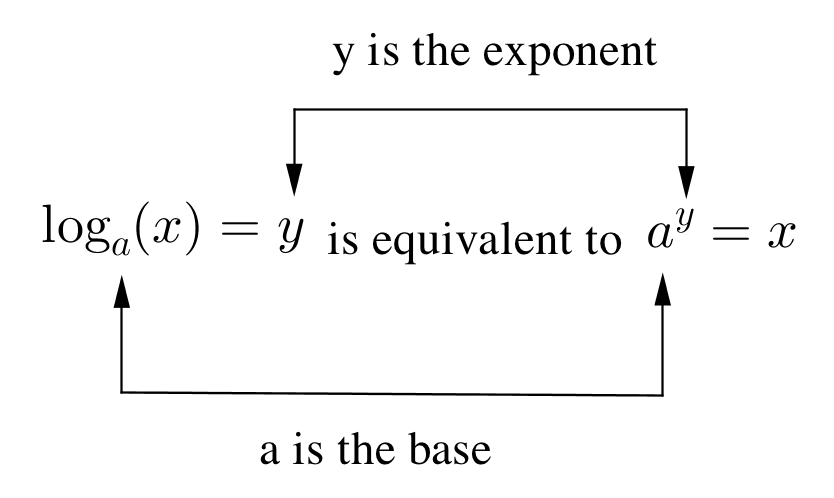
\includegraphics{logdef}} \end{tabular} & \begin{tabular}{c } Example: $f(x) = \log_2(x)$ \\ \scalebox{.7}{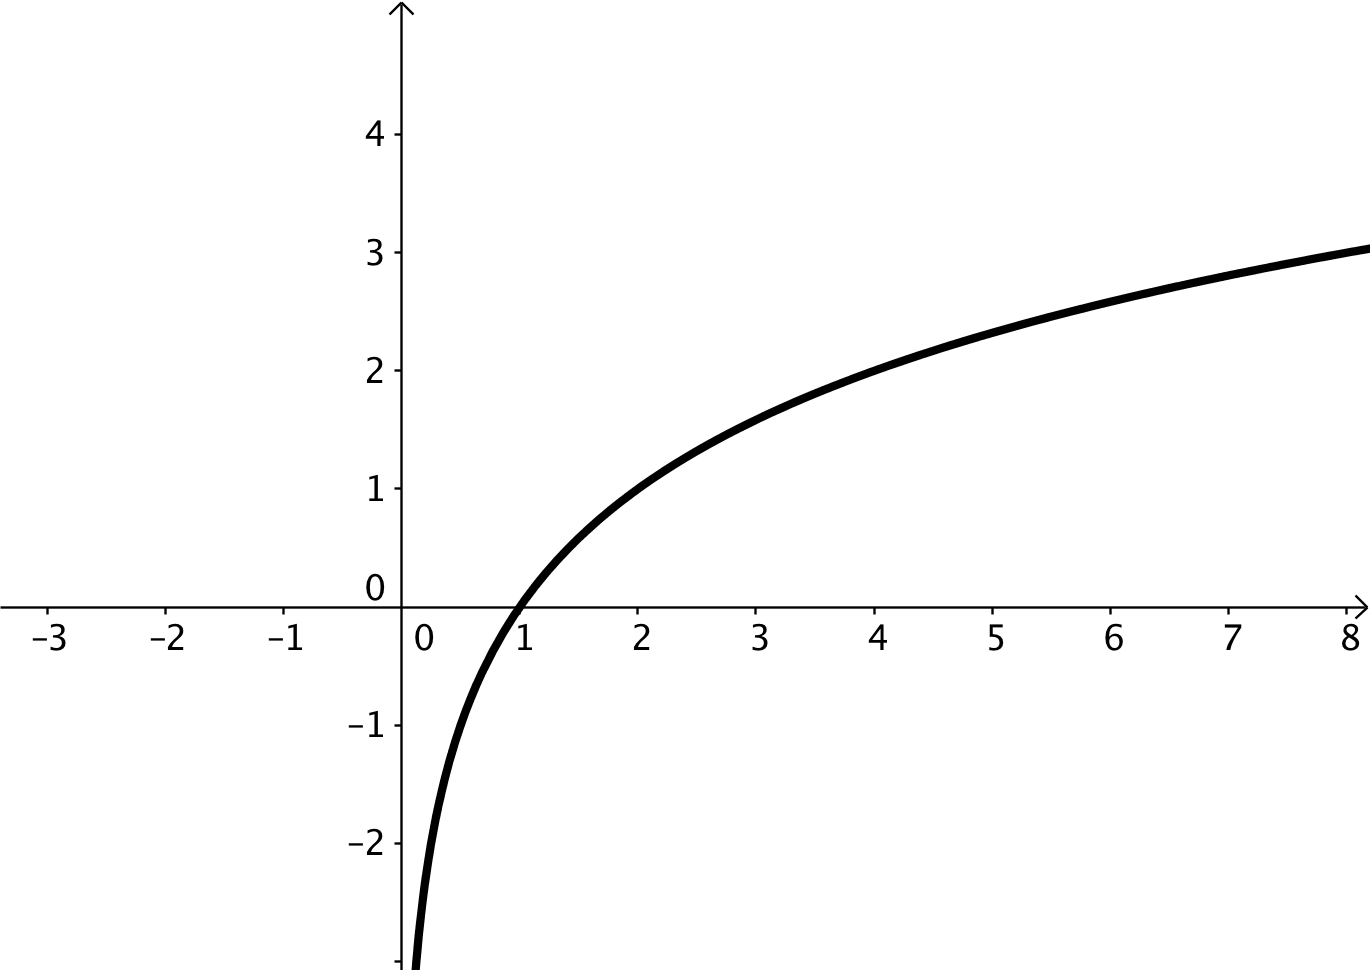
\includegraphics{log1}} \end{tabular}
\end{tabular}

\begin{enumerate}
\item Write in exponential form.  \\
model: $\log_a(x)=y$ \hspace{1in} $\log_2 (16) = 4$ \hspace{1in} $\log_p (13) = y$\\[1in]

\item Write in logarithmic form. \\
model: $a^y = x$  \hspace{1in} $4^{-3} = \dfrac{1}{64}$ \hspace{1in} $\pi^t = 9.4$ \\[.5in]


\item The expression $\log x$, called the \emph{common logarithm}, is shorthand for $\log_{10}(x)$. Write in logarithmic form: $10^{2x+3} = 7$. \\[.5in]


\item The expression $\log x$, called the \emph{common logarithm}, is shorthand for $\log_{10}(x)$. Write in logarithmic form: $10^{2x+3} = 7$. \\[.5in]

\item Find the domain of the function $f(x) = \ln (9-6x)$. \\[.8in]



\subsection{Evaluating Logarithmic Expressions}
  
\item Find the number, if possible. Rewrite in exponential form, either to solve, or to check.
$\log_2 \left(  \dfrac{1}{8} \right)$  \hspace{1in} $\log_3 (27)$  \hspace{1in} $\log_4(0)$   \hspace{1in} $\log_b\left(\dfrac{1}{b^3}\right)$ \\[1in]




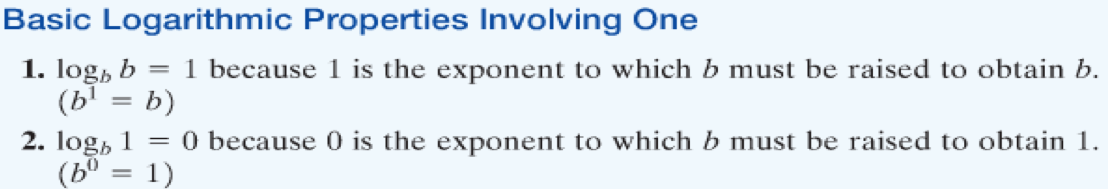
\includegraphics[scale=.9]{logprop1}
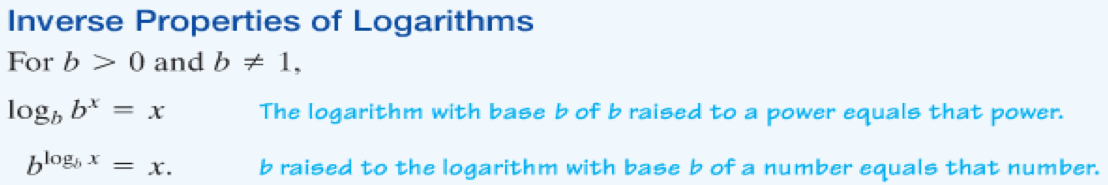
\includegraphics[scale=.9]{logprop2}

\item Evaluate the common and natural logarithms.\\
$\log (100,000)$  \hspace{1in} $\log (0.001)$  \hspace{1in} $\ln (e^4)$   \hspace{1in} $\ln \left(\dfrac{1}{e}\right)$ \\

\subsection{Graphing Logarithmic Functions} ~

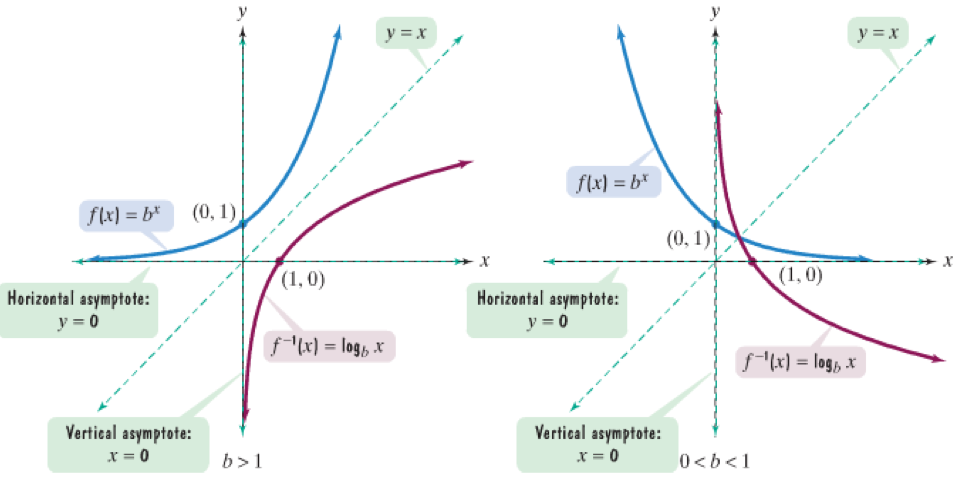
\includegraphics{loggraph}

\item Graph $\log_2 x$ and $\log_{1/4} x$\\
\begin{center}
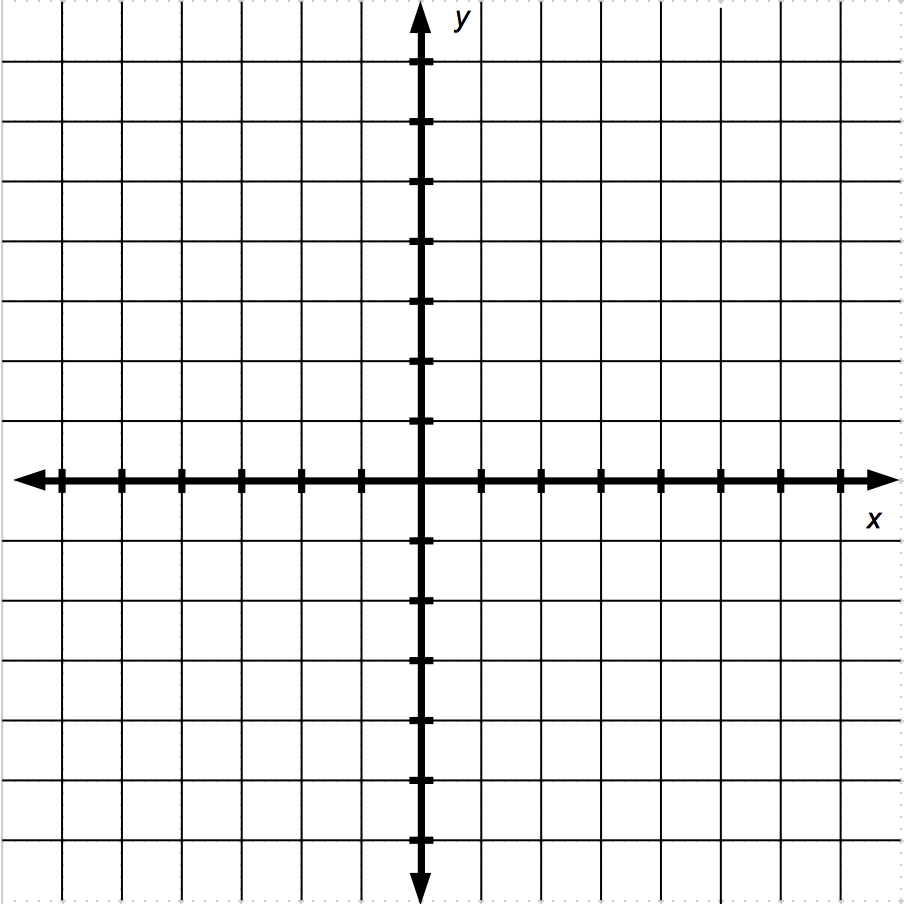
\includegraphics[scale=.4]{bigaxes}
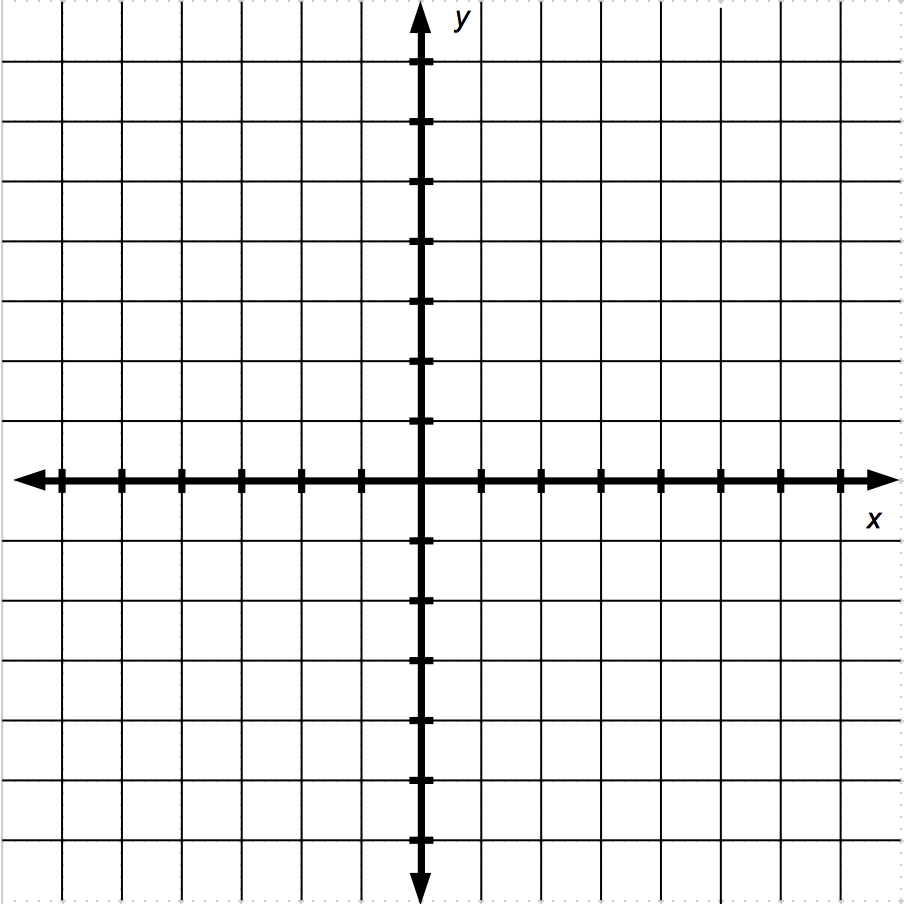
\includegraphics[scale=.4]{bigaxes}\vfill
\end{center}

\end{enumerate}

\noindent \textbf{Student Learning Outcomes Check}

\begin{enumerate}
\item Can you recognize a logarithic function graphically and algebraically?
\item Can you evaluate the logarithmic expressions?
\item Are you able to apply basic logarithmic properties?

\end{enumerate}

\noindent \textbf{If any of your answers were no, please ask about these topics in class.}


